\documentclass[../mech.tex]{subfiles}
\graphicspath{{\subfix{../figures/}}}
\begin{document}
\chapter{Linear Momentum}
\section{Linear Momentum}
Linear momentum is defined by the equation:
\[ \vec{p}=m\vec{v} \]
Momentum is a vector quantity and has the same direction as the velocity.

Momentum can be used to analyze collisions and explosions.
\begin{itemize}
    \item A collision is a model for an interaction where the forces exerted between the involved objects in the system are much larger than the net external force exerted on those objects during the interaction.
    \item An explosion is a model for an interaction in which forces internal to the system move objects within that system apart.
\end{itemize}

\begin{example}
    (a) Derive an expression for the kinetic energy of an object in terms of momentum.

    Substitute $p=mv$ into $K=\frac{1}{2}mv^2$ to get $K=\frac{p^2}{2m}$.

    (b) Derive an expression for the momentum of an object in terms of kinetic energy.

    We get that $v=\sqrt{\frac{2k}{m}}$. Substituting this into $p=mv$ gives $p=\sqrt{2mk}$.
\end{example}

\ex A moving block of mass $m_0$ has kinetic energy $K_0$ and momentum of magnitude $p_0$. A second block of mass $2m_0$ is moving with the same kinetic energy $K_0$. What is the magnitude of the momentum of the second blocK?

\ex A student is pulling a cart full of water horizontally on flat ground at a constant velocity. The cart has a small hole through which the water slowly leaks out of the cart. For the system consisting of the cart and the water within the cart, how is the magnitude of the momentum of the system changing, if at all?

\section{Change in Momentum and Impulse}
The rate of change of a system's momentum is equal to the net external force exerted on that system.
\[ F_{NET}=\frac{\dd \vec{p}}{\dd t} \]
Impulse is defined as the integral of a force exerted on an object or system over a time interval.
\[ J = \int F(t)\dd t \]
Impulse is a vector quantity and has the same direction as the net force exerted on the system.

Change in momentum is the difference between a system's final momentum and its initial momentum.
\[ \Delta \vec{p} = \vec{p}_f-\vec{p}_i \]

The impulse-momentum theorem relates impulse delivered to an object and the object's change in momentum.
\[ \vec{J}=\Delta \vec{p} \qquad \int F(t)\dd t = m\Delta \vec{v} \]

\begin{example}
    The net force $F$ acting on an object that moves along a straight line is given as a function of time $t$ by $F(t)=\kappa t^2+\tau$, where $\kappa = 2$N/s$^2$ and $\tau=4$N. What is the change in momentum of the object from $t=0$ s to $t=3$ s?

    Integrate $F(t)\dd t$ from $0$ to $3$ to get $\Delta \vec{p} = 59$ N$\cdot$m.
\end{example}

\ex A 50-kg student sitting in a rolling chair at rest pushes against a wall, which applies a 10 N$\cdot$s horizontal impulse to the student. Later, a 40-kg student is at rest in the same rolling chair and catches a 10-kg ball while applying a 10 N$\cdot$s horizontal impulse to the ball. 
Describe the students' final speeds and provide a valid reasoning to support this claim.

\ex \begin{center}
    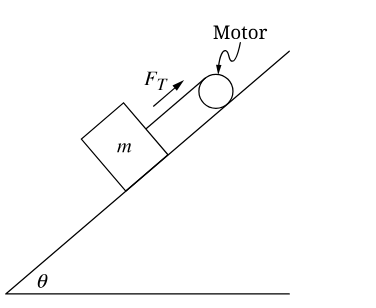
\includegraphics[width=0.5\textwidth]{4.1.PNG}
\end{center}
A block of mass $m$ can move with negligible friction on a ramp that is at an angle $\theta$ from the horizontal, as shown in the figure. Starting at time $t=0$, the motor creates a varying string tension $F_T$ given by $F_T=2kt$, where $k$ is a positive constant.
If the positive direction is taken to be up the ramp, what is the magnitude of the impulse exerted on the block between $t_1>0$ and a later time $t_2$?

\section{Conservation of Linear Momentum}
A collection of objects with individual momenta can be described as one system with one center of mass velocity.
\begin{itemize}
    \item The velocity of a system's center of mass can be calculated using the equation 
    \[ v_{cm}=\frac{\sum m_iv_i}{\sum m} \]
\end{itemize}
The total momentum of a system is the sum of the momenta of the system's constituent parts.

In the absence of net external forces, any change to the momentum of an object within a system must be balanced by an equivalent and opposite change of momentum elsewhere within the system.

Momentum is conserved in all interactions.

If the net external force on the selected system is zero, the total momentum of the system is constant.

If the net external force on the selected system is nonzero, momentum is not transferred between the system and the environment.

\pagebreak
\begin{example}
    An object of mass $m$ is moving with speed $v_0$ to the right on a horizontal frictionless surface, when it explodes into two points. Subsequently, one piece of mass $(2/5)m$ moves with a speed $v_0/2$ to the left. What is the speed of the other piece of the object?

    We know momentum before has to equal the momentum after.

    So we get $mv_0=\frac{3}{5}mv_f-\frac{2}{5}m\frac{v_0}{2}$. Solving for $v_f$ gives $v_f=2v_0$.
\end{example}

\ex In three different scenarios, a student of mass $3m$ pulls on a lightweight rope attached to a block of mass $m$. The student and the block are both initially at rest in each scenario.
In Scenario 1, the student stands on the shore of a frozen lake and the block is on the ice. After the student starts pulling on the rope in Scenario 1, the block slides with negligible friction while the student remains in the same location on the shore.
In Scenario 2, both the student and the block are on the ice. After the student starts pulling the rope in Scenario 2, both the student and the block slide with negligible friction. In Scenario 3, the block is at rest on the shore while the student is on the ice.
After the student starts pulling on the rope in Scenario 3, the student slides with negligible friction while the block remains in the same location on the shore. The final velocity of the block relative to the student is the same in each scenario.
Which scenario, if any, is the final speed of the center of mass of the block-student system the greatest?

\ex \begin{center}
    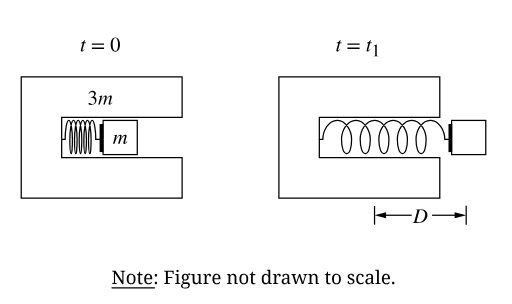
\includegraphics[width=0.5\textwidth]{4.3.PNG}
\end{center}
A small block of mass $m$ is held in place inside a larger, U-shaped block of mass $3m$, as shown in the figure. Initially, the centers of mass of the two blocks are located at the same position, and a spring 
attached to the larger block is compressed a distance $D$ from its relaxed length by the smaller block. At time $t=0$, the two blocks are released from rest. At time $t_1>0$, the spring is at its relaxed length, the centers of mass of the two blocks are a distance $D$ apart, and the small block is moving 
to the right with a velocity $v$ just as it loses contact with the spring. If there are no external forces exerted on the block-spring system, what is the distance of separation of the two centers of mass at a later time $t>t_1$?

\section{Elastic and Inelastic Collisions}
An elastic collision between objects is one in which the initial kinetic energy of the system is equal to the final kinetic energy of the system.

In an elastic collision, the final kinetic energies of each of the objects within the system may be different from their initial kinetic energies.

An inelastic collision between objects is one in which the total kinetic energy of the system decreases.

In an inelastic collision, some of the initial kinetic energy is not restored to kinetic energy but it is transformed by nonconservative forces into other forms of energy.

In a perfectly inelastic collision, the objects stick together and move the same velocity after the collision.

\pagebreak
\begin{example}
    A child of mass $20$ kg who is running at a speed of $4.0$ m/s jumps onto a stationary sled of mass $5.0$ kg on a frozen lake. What is the speed at which the child and sled begin to slide across the ice?

    From inelastic collision formula, we get $m_1v_{1B}=(m_1+m_2)v_f$. So, we get $v_f=\frac{m_1v_{1B}}{m_1+m_2}=\frac{80}{25}=3.2$ m/s.
\end{example}

\ex \begin{center}
    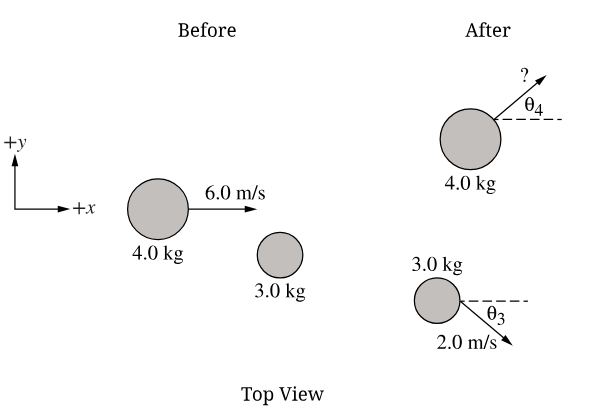
\includegraphics[width=0.5\textwidth]{4.4.PNG}
\end{center}
Two pucks are free to slide on a horizontal surface with negligible friction. The figure shows a top view of the pucks, one of mass $4.0$ kg and one of mass $3.0$ kg, before and after they undergo an elastic collision with each other.
Before the collision, the $4.0$-kg puck slides at $6.0$ m/s in the $+x$-direction and the $3.0$-kg puck is at rest. After the collision, the $3.0$-kg puck moves with a speed of $2.0$ m/s at an unknown angle 
$\theta_3$ measured clockwise from the $+x$-direction, as indicated, while the $4.0$-kg puck moves at an unknown speed and at an unknown angle $\theta_4$ measured counterclockwise from the $+x$-direction, as indicated. What is the speed of the $4.0$-kg puck after the elastic collision.

\ex Students perform an experiment with mutiple trials using blocks that can slide with negligible friction on a straight, horizontal track. In each trial, a block of mass $m_1$ slides with speed $v_1$ on the track and collides with a stationary block of mass $m_2$.
The blocks stick together and move with speed $v_f$ after the collision. In each trial, $m_1$ and $v_1$ are kept constant but the mass $m_2$ of the stationary block is varied, and $v_f$ is recorded. The students graph $v_f$ as a function of $m_2$.
Graph a best-fit curve to the data collected by the students.

\end{document}